\documentclass[12pt,a4paper,x11names]{article}
\usepackage[utf8]{inputenc}
\usepackage{amsmath}
\usepackage{amsfonts}
\usepackage{amssymb}
\usepackage[top=0.8cm, bottom=0.8cm, left=0.8cm, right=0.8cm, includehead, includefoot, heightrounded]{geometry}
\usepackage{pagecolor}
\usepackage{fancyhdr}
\usepackage[style=ieee,sorting=none,url=true,doi=true]{biblatex}
\usepackage{tikz}
\usetikzlibrary{arrows.meta}
\usetikzlibrary{automata, shapes}
\usetikzlibrary{decorations.markings}
\usetikzlibrary{calc}
\usepackage{pdflscape}
\usepackage{makecell}
\usepackage{hhline}
\usepackage{tabularx}
\usepackage{booktabs}
\usepackage{titlesec}
\usepackage{ltablex}
\usepackage{minted}
\usepackage{caption}
\usepackage{subcaption}
\usepackage{multirow}
\pagestyle{fancy}

\addbibresource{refs.bib}

\definecolor{lightblue}{HTML}{F7FAFC}
\definecolor{blue}{HTML}{3182ce}
\definecolor{darkblue}{HTML}{2a4365}
\pagecolor{lightblue}

\setlength{\headheight}{15pt}
\addtolength{\topmargin}{-3pt}

\usepackage[defaultfam,tabular,lining]{montserrat}
\usepackage[T1]{fontenc}
\renewcommand*\oldstylenums[1]{{\fontfamily{Montserrat-TOsF}\selectfont #1}}


\titlespacing*{\paragraph}{0pt}{0.5ex plus 1ex minus .2ex}{1em}

\lfoot{\textcopyright \ \ Q Misell 2021}
\cfoot{\thepage}
\rfoot{}

\author{Q Misell}
\title{A participant-based evaluation of the UI of My5}

\begin{document}

\maketitle{}
\tableofcontents{}
\newpage{}

\section{Abstract}

\section{Introduction}
Many TV broadcasters offer video on demand services, which contribute to a sizeable percentage of the TV market globally\cite{ofcom-uk-vod-market}. As more and more people move towards on demand services over liner TV it is vital that broadcasters remain competitive with their VoD offering.

I have been asked to conduct an evaluation of Channel 5 TV company's My5 video on demand streaming service, to asses the usability of their service. The evaluation will be conducted in the form of a comparison with competitor video on demand services to gauge My5's usability in relation with the market, and to note where others have excelled My5, to provide opportunities for learning. The evaluation will be used to ensure Channel 5's position in the video on demand market remains competitive.

\section{Evaluation strategy}
The primary purpose of this evaluation is to consider how Channel 5's offering compares to the rest of the VoD market. The BBC iPlayer was chosen as a competitor with a similar offering to compare against. The BBC has the highest market VoD penetration of any traditional broadcaster in the UK - 28\% - although this is far behind some competitors such as Netflix at 66\%\cite{ofcom-bbc-report}. It was decided to go with the BBC over Netflix, as Netflix's offering is too different from that of Channel 5's My5 and the BBC's iPlayer to be able to effectively conduct an A/B test. The BBC's online offering is also rated highly by audiences in comparison to alternative services\cite{ofcom-bbc-performance}, so will offer a good benchmark for a market leading VoD service. The comparison between the two services was conducted with a System Usability Scale and an A/B test.

\subsection{System Usability Scale}
One of the best ways to identity pain points with a UI is by interviewing people, we can follow up on unexpected responses and dig deeper into problems identified. However, due to time constraints and the current difficulty of organising the type of in person interaction required for a good interview under Covid-19, a remote questionnaire was chosen. A questionnaire streamlines the analysis process, especially if numerical responses are given to questions, however constructing an effective but simple questionnaire is a surprisingly difficult task\cite{designing-user-experience}. 

A Likert scale\cite{likert1932} is often used to collect perceptions of a system through rating scales, usually utilising a five point scale from `strongly agree' to `strongly disagree'. The System Usability Scale is a ``robust and reliable"\cite{sus} which is particularly suited to the task at hand, both with its ability to be automatically scored (using a spread-sheeting programme) and its simplicity for participants to use. The SUS correlates well with other, more complicated, usability scales. Additionally the SUS is also available to use free of charge, unlike some other usability questionnaires, with only a reference to the original source.

\subsection{A/B testing}
A/B testing is representative of real world usage, as compared to lab based inspections which can result in artificial or contrived results not representative of how the user may have acted unguided in the real world\cite{firmenich2019usability}. As the objective here is to analyse the real world usability of a VoD platform, and users are not expected to read a manual etc. before starting to use a VoD platform entirely new to them an unsupervised A/B test is the most suitable for this. 

\section{Research methodology}
\textit{Google Forms} was used to collect responses from participants, it is a service participants will likely already be familiar with how to use, and has an intuitive and no nonsense form interface. It also allows providing blocks of text in-between questions, which where used to provide instructions about tasks to complete on the websites under evaluation before continuing with responding to the survey. \textit{Google Forms} additionally provides some useful advanced features, such as randomisation of page order, which was used to have 50\% of participants evaluate Channel 5's service first, and the other evaluate the competitor first. Google is a market leader in accessible web technology, so the form will be accessible to those who use screen readers, or other common technology to access their computer in a way that works for them.

The lack of control in a remote unsupervised test was seen as a benefit to this study, as it provides opportunity for more natural behaviour when interacting with the systems under test, as opposed to the artificial results than can result from lab-based studies. The tests where conducted against the live versions of the services available at \url{https://my5.tv} and \url{https://www.bbc.co.uk/iplayer}. This ensures the test data and interaction fidelity is representative of the actual product, and not some stripped down version contrived exclusively for this test. As users are being left unsupervised when interacting with the services there is a risk that users may come across content upsetting to them. There will be nothing illegal or extremely explicit on these services, as they're regulated by the Ofcom broadcasting code\cite{ofcom-broadcasting-code}. Both services also provide warnings before watching any content that may be unsuitable for some audiences, regardless all participants where over 16 and voluntarily agreed to take part.

\subsection{A/B testing design}
The interface of the two VoD services was evaluated through a completion of the same set of tasks on both systems. This ensures the results are comparing the usability of the two systems, and not on the relative difficulty of different tasks. The testing was completed using a \textit{within-groups} experiment. This is suited best for simple tasks with a low learning curve, such at the systems under test\cite{lewistask}. It has certain disadvantages with using the same users to test both systems, in that there might be advantages or disadvantages to having completed a similar task before. As stated above the \textit{Google Forms} page randomisation feature will be used to show some users My5 first, and others the iPlayer first. 

\subsection{SUS}
The participants where presented with the SUS questions and a liner scale 1-5 from strongly disagree to strongly agree, as shown below.

\begin{center}
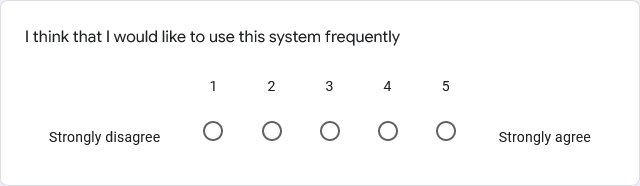
\includegraphics[scale=0.5]{sus-screenshot.png}
\end{center}

None of the SUS questions where required, and this was communicated to the participants in the notes accompanying the questionnaire. If a participant felt they couldn't answer a question a score of 3 was given for the final score calculation\cite{sus}.

The questions in the SUS alternate between questions designed to elicit a positive response, with those designed to elicit a negative response. This engages the participant and attempts to eliminate inadvertent bias; e.g. in always selecting responses closer to 5.

For odd numbered questions their score is the scale position minus 1, whereas for even questions it is 5 minus the scale position. These individual question scores can then be summed and multiplied by 2.5 to give a final SUS score from 0 to 100.

\subsection{User tasks}
Four tasks where selected to be given to users to complete, representing the primary features common to both platforms. The tasks chosen where:

\begin{enumerate}
\item Watch a specific programme; on My5 this was chosen to be `London's Greatest Bridges' episode 4, on the iPlayer the chosen programme was `The Graham Norton Show' series 29, episode 20.
\item Watch live TV; on My5 participants where asked to watch 5Select, on the iPlayer it was BBC Parliament.
\item Find out when a programme is on; on My5 find what is on at 7pm tomorrow on 5Action, on the iPlayer find what is on at 7pm tomorrow on BBC Scotland.
\item Find a programme of your choosing and add it to `My List' on My5 and `My Programmes' on the iPlayer.
\end{enumerate}

Tasks will be completed in the same order with all users, and are roughly in order of increasing difficulty\cite{lewistask}. Users will not be provided with instructions on how to complete the tasks, as they would be hitting the systems cold in a real life scenario. Users where asked if they managed to complete each task, as a rough gauge of both task difficulty and the usability of both systems in respect of individual tasks.

\subsection{Participants}
We where strictly prohibited from conducting this study with the general public. The survey was sent out to friends and acquaintances in various society chat groups (e.g. Discord). There is a good mix of people and backgrounds in University societies. The sample was however self selecting in some ways, as it was sent out as an open invitation with no obligation to complete, it was however expected that a mostly uniform distribution of characteristics would appear, with the exception of computer proficiency, which would tend towards the more proficient end of the spectrum due to how the invitation to participate was given.

Some basic questions where placed at the start of the questionnaire to gather background information about the participants, some objective such as age, native English speaker status, etc., some more subjective such as to rate their perceived proficiently with computers.

\subsection{Data analysis}
The responses from \textit{Google Forms} are provided in the form of a \textit{Google Sheets} spreadsheet, which can easily be exported to a CSV file for analysis. The data was processed, analysed, and rendered in Python; using Pandas for processing and statistical analysis and Matplotlib for graph rendering. 

\subsection{Pilot testing}
Whilst conducting pilot testing the questionnaire was overall rated as easy to understand and follow by pilot participants. A few issues where however raised, primarily that it wasn't clear that a My5 and BBC account where required to complete some of the tasks, and that it was not clear to participants that such accounts where free to create. A notice about this was added to the questionnaire, drawing attention to the free nature of these accounts. It was also raised by one pilot participant that not everyone will have the TV license required to access the iPlayer, so some advice was added regarding this, suggesting that if one does not have a TV license they may wish to complete this questionnaire at a friend's house who does have a TV license, to be in compliance with the law.

\section{Results}
13 people participated in this study, with a 100\% response rate. Participants where aged between 17 and 50, and 85\% where native English speakers. Most rated their proficiency with computers as 4 (on a scale of 1-5), with only 2 choosing a lower scoring. This is likely due to the way the participants where recruited, that being using internet communications, so people would have to be fairly competent with computers in the first place to receive the invitation. 77\% of participants had used the iPlayer previously, whilst only 54\% had previously used My5. 46\% participated using a mobile phone, 38\% on a laptop, and 15\% on a desktop computer. 

\begin{figure}[!h]
\begin{minipage}[c]{.5\linewidth}
\caption{Self rated computer proficiency of the participants}
\centering
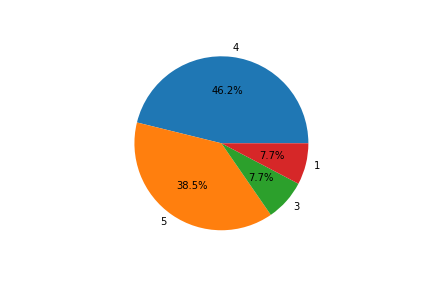
\includegraphics[width=\textwidth]{plots/proficiency.png}
\end{minipage}
\hfill
\begin{minipage}[c]{.5\linewidth}
\caption{Age of the participants}
\centering
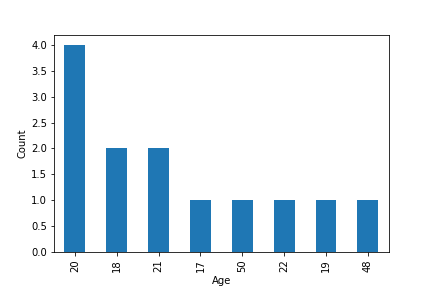
\includegraphics[width=\textwidth]{plots/age.png}
\end{minipage}
\end{figure}

The table below summaries the overall SUS scores for both platforms, as well as the SUS scores for some groups of participants. My5 is rated higher than the iPlayer, and of particular note is that those who had not used My5 before gave it a much higher rating than those who had not used the iPlayer before. There is not notable difference in ease of use between native and non-native English speakers.

\begin{center}
\begin{tabular}{l|l||r|r|r|r|r}
    Platform & Group & Count & Mean & Std. dev. & Min & Max \\
    \hline
    \multirow{5}{*}{My5} & Total & 13 & 74.42 & 17.74 & 45.0 & 100.0 \\
    & Used My5 before & 6 & 77.92 & 17.92 & 52.5 & 92.5 \\
    & Hadn't used My5 before & 7 & 71.43 & 18.42 & 45.0 & 100.0 \\
    & Native English speaker & 11 & 70.91 & 16.78 & 45.0 & 92.5 \\
    & Non-native English speaker & 2 & 93.75 & 8.84 & 87.5 & 100.0 \\
    \hline
    \multirow{5}{*}{iPlayer} & Total & 13 & 63.65 & 25.30 & 7.5 & 97.5 \\
    & Used the iPlayer before & 10 & 72.00 & 18.29 & 47.5 & 97.5 \\
    & Hadn't used the iPlayer before & 3 & 35.83 & 28.75 & 35.0 & 65.0 \\
    & Native English speaker & 11 & 65.05 & 27.18 & 7.5 & 97.5 \\
    & Non-native English speaker & 2 & 72.50 & 10.60 & 65.0 & 80.0 \\
    \hline
\end{tabular}
\end{center}

\begin{figure}
\centering
\begin{subfigure}[b]{0.45\linewidth}
\centering
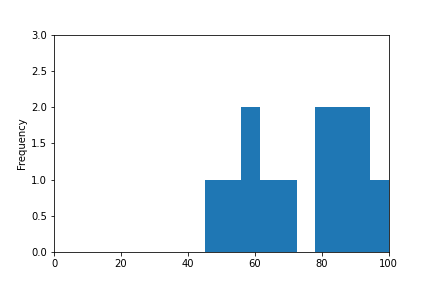
\includegraphics[width=\textwidth]{plots/my5-sus.png}
\caption{My5 SUS}
\end{subfigure}
\hfill
\begin{subfigure}[b]{0.45\linewidth}
\centering
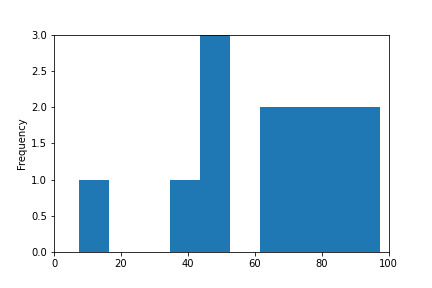
\includegraphics[width=\textwidth]{plots/iplayer-sus.png}
\caption{iPlayer SUS}
\end{subfigure}
\caption{Frequency distribution of the SUS scores}
\end{figure}

A paired samples t-test was conducted with a threshold value of $0.05$ to determine if any significant difference existed between the two interfaces. The t-value between the two SUS scores is $1.567$ with a p-value of $0.143$. This is not significant enough to reject the null hypothesis, and therefore we must conclude there is no significant difference between My5 and the iPlayer in terms of usability.

Additional ANOVA tests where performed, using previous experience with My5/iPlayer as the factor. Between those who had not used the iPlayer before and those who had the F-value is $7.119$ with a p-value of $0.022$. For My5 the F-value is $0.140$ with a p-value of $0.716$.

\section{Conclusions}

\newpage{}
\printbibliography[title=Bibliography,heading=bibintoc]{}

\appendix{}

\section{Questionnaire}
\subsection{Basic questions}
\begin{itemize}
\item How old are you?
\item Are you a native English speaker?
\item How would you rate your proficiency with computers?
\item Have you used My5 before?
\item Have you used the iPlayer before?
\item On what device will you be partaking in this evaluation?
\end{itemize}

\subsection{BBC iPlayer}
Instructions given:
\begin{quote}
Please complete the following tasks on the BBC iPlayer (available at \url{https://www.bbc.co.uk/iplayer}), in the order that they are given.

\begin{enumerate}
\item Find and start watching 'The Graham Norton Show' series 29, episode 20.
\item Watch BBC Parliament live.
\item Find out what is on at 7pm tomorrow on BBC Scotland.
\item Find a programme of your choosing and add it to 'My Programmes'.
\end{enumerate}
\end{quote}

\noindent{}Questions:
\begin{itemize}
\item Please tick all tasks that you managed to complete successfully
\item I think that I would like to use this system frequently
\item I found the system unnecessarily complex
\item I thought the system was easy to use
\item I think that I would need the support of a technical person to be able to use this system
\item I found the various functions in this system were well integrated
\item I thought the was too much inconsistency in this system
\item I would imagine that most people would learn to use this system very quickly
\item I found the system cumbersome to use
\item I felt very confident using the system
\item I needed to learn a lot of things before I could get going with this system
\end{itemize}

\subsection{My5}
Instructions given:
\begin{quote}
Please complete the following tasks on My5 (available at \url{https://my5.tv}), in the order that they are given.

\begin{enumerate}
\item Find and start watching 'London's Greatest Bridges' episode 4.
\item Watch 5Select live.
\item Find what is on at 7pm tomorrow on 5Action.
\item Find a programme of your choosing and add it to 'My List'.
\end{enumerate}
\end{quote}

\noindent{}Questions:
\begin{itemize}
\item Please tick all tasks that you managed to complete successfully
\item I think that I would like to use this system frequently
\item I found the system unnecessarily complex
\item I thought the system was easy to use
\item I think that I would need the support of a technical person to be able to use this system
\item I found the various functions in this system were well integrated
\item I thought the was too much inconsistency in this system
\item I would imagine that most people would learn to use this system very quickly
\item I found the system cumbersome to use
\item I felt very confident using the system
\item I needed
\end{itemize}

\end{document}